\chapter{Project Plan}
\label{ch:project_plan}
In the following section, the project plan of the proposed master's thesis is discussed.
The project plan consists of a work plan, time schedule, and risk assessment.
The work plan defines the project objectives, milestones, tasks, and deliverables and is presented in \autoref{sec:work_plan}.
The time schedule represents the mapping of the proposed work plan to calendar weeks and is discussed in \autoref{sec:time_schedule}.
The risk assessment evaluates technical and non-technical risks for the proposed project plan and is discussed in \autoref{sec:risk_assessment}.

\section{Work Plan}
\label{sec:work_plan}
%\todo{Workplan, Incremental Parts ("inkremente"), Dependencies, Deliverable-Duration-Limitation, time schedule (milestones, temporal dependencies)}
The work plan structures the proposed thesis into six milestones.
Each milestone represents a major phase of the proposed master's thesis.
The milestones serve as intermediate project goals which enable monitoring and reporting of project progress.
Each milestone is defined by its duration in Calendar Weeks (CW), deliverables, and tasks.
Each milestone consists of at least one task.
A task of a milestone is referred to as increment.
The duration of a milestone depends on the duration of its increments and increment interdependencies.
The projected timescales for the completion of milestones and increments have been calculated based on empirical values.
The milestones of the proposed master's thesis are defined as follows:
\begin{description}
    \item[Milestone I:] Preliminary Work
    \begin{description}[style=multiline, leftmargin=\widthof{\textbf{Deliverables:}}]
        \item[Duration:] 14 Weeks (15. April 2024 (CW 16) -- 22. July 2024 (CW 30))
        \item[Deliverables:] Master's thesis proposal
    \end{description}
    \item[Milestone II:] Realization
    \begin{description}[style=multiline, leftmargin=\widthof{\textbf{Deliverables:}}]
        \item[Duration:] 9 Weeks (22. July 2024 (CW 30) -- 23. September 2024 (CW 39))
        \item[Deliverables:]
        \begin{enumerate}[label=\alph*), leftmargin=\widthof{a)}+\labelsep]
            \item Software Design, Implementation, Tests (Unit, Integration, and System), \& Test Coverage Report of CASC-SAS
            \item Hardware Deployment Scripts of CASC-SAS
            \item Thesis Chapter: Realization
        \end{enumerate}
        \item[Increments:]
        \begin{enumerate}[label=\arabic*), leftmargin=\widthof{a)}+\labelsep]
            \item Design, Implementation, Tests, \& Deployment of CASA (8 Weeks)
            \item Design, Implementation, Tests, \& Deployment of SABAAC (8 Weeks)
            \item Architecture \& Code Review (Optional, Single Meeting)
            \item Writing of Documentation (5 Weeks)
        \end{enumerate}
    \end{description}
    \item[Milestone III:] Evaluation
    \begin{description}[style=multiline, leftmargin=\widthof{\textbf{Deliverables:}}]
        \item[Duration:] 9 Weeks (23. September 2024 (CW 39) -- 25. November 2024 (CW 48))
        \item[Deliverables:]
        \begin{enumerate}[label=\alph*), leftmargin=\widthof{a)}+\labelsep]
            \item Evaluation Results of CASC-SAS
            \item Thesis Chapter: Evaluation
        \end{enumerate}
        \item[Increments:]
        \begin{enumerate}[label=\arabic*), leftmargin=\widthof{a)}+\labelsep]
            \item Security Evaluation (9 Weeks)
            \item Performance Evaluation (9 Weeks)
            \item Economic Evaluation (5 Weeks)
            \item Writing of Documentation (4 Weeks)
        \end{enumerate}
    \end{description}
    \item[Milestone IV:] Conclusion
    \begin{description}[style=multiline, leftmargin=\widthof{\textbf{Deliverables:}}]
        \item[Duration:] 2 Weeks (25. November 2024 (CW 48) -- 09. December 2024 (CW 50))
        \item[Deliverables:]
        \begin{enumerate}[label=\alph*), leftmargin=\widthof{a)}+\labelsep]
            \item Thesis Chapter: Conclusion
            \item Thesis Chapter: Limitations
            \item Thesis Chapter: Future Work
            \item Thesis Chapter: Abstract
        \end{enumerate}
        \item[Increment:] Writing of Documentation: Conduct a review of results and derive a conclusion, limitations, and future work with regard to the research questions (2 Weeks)
    \end{description}
    \item[Milestone V:] Review
    \begin{description}[style=multiline, leftmargin=\widthof{\textbf{Deliverables:}}]
        \item[Duration:] 5 Weeks (09. December 2024 (CW 50) -- 13. January 2025 (CW 03))
        \item[Deliverables:] Reviewed \& Proofread Master's Thesis
        \item[Increments:]
        \begin{enumerate}[label=\arabic*), leftmargin=\widthof{a)}+\labelsep]
            \item Internal Review: Proofreading \& Correction by the Authors (2 Weeks)
            \item External Review: Proofreading \& Correction by External Readers (4 Weeks)
        \end{enumerate}
    \end{description}
    \item[Milestone VI:] Finalization
    \begin{description}[style=multiline, leftmargin=\widthof{\textbf{Deliverables:}}]
        \item[Duration:] 6 Weeks (09. December 2024 (CW 50) -- 20. January 2025 (CW 04))
        \item[Deliverables:]
        \begin{enumerate}[label=\alph*), leftmargin=\widthof{a)}+\labelsep]
            \item Printed \& Bound Master's Thesis
            \item Master's Thesis Presentation Slides
        \end{enumerate}
        \item[Increments:]
        \begin{enumerate}[label=\arabic*), leftmargin=\widthof{a)}+\labelsep]
            \item Thesis Presentation Preparation (5 Weeks)
            \item Printing \& Binding of Thesis (1 Weeks)
        \end{enumerate}
    \end{description}
\end{description}

\section{Time Schedule}
\label{sec:time_schedule}
The time schedule maps the milestones and increments as defined in \autoref{sec:work_plan} to specific calendar weeks.
The mapping of the proposed master's thesis is shown in \autoref{fig:timeplan}.
The proposed time schedule covers the period from the 30th calendar week of 2024 to the 4th calendar week of 2025.
In other words, the time schedule spans from July 22nd, 2024 to January 20th, 2025.
The work plan stipulates that the approach presented in this thesis proposal has to be realized and evaluated within the 26-week period.
Additionally, the remaining chapters must be completed and the written elaboration of the thesis must be finalized within this timeframe.

The visualized time schedule shown in \autoref{fig:timeplan} illustrates the milestones II to VI.
The initial milestone represents the preliminary work and has therefore been excluded from the visual representation.
Multiple increments mapped to the same calendar weeks may be performed in parallel, as there are either no interdependencies or existing dependencies can be resolved beforehand.
Accordingly, the indicated duration of an increment takes the occurrence of parallelization into account.
In regard to the realization of CASA and SABAAC, the dependency inversion principle and service interfaces are employed to resolve existing dependencies.
Other increments such as the different areas of the evaluation do not have interdependencies.
The realization, evaluation, and conclusion milestones depend on the results of their predecessors.
Consequently, the preceding milestones must be completed before the next milestone can commence.
The finalization milestone is only partially dependent on the review milestone due to its binding increment.
Accordingly, independent increments of these milestones can be performed simultaneously.
\begin{figure}
    \centering
    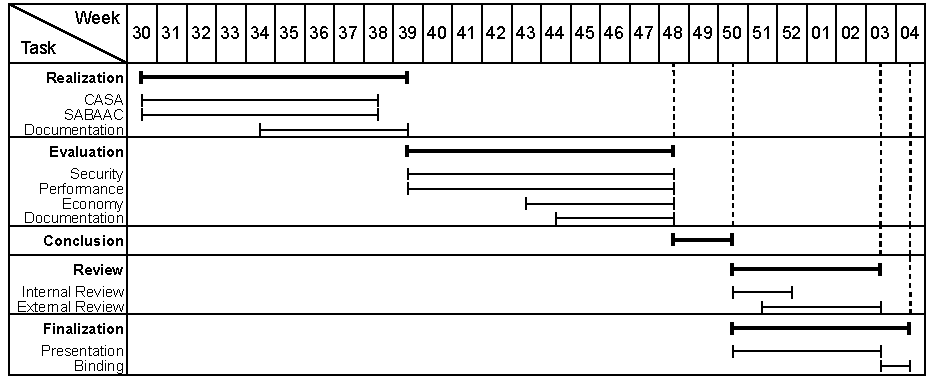
\includegraphics[width=1.0\linewidth]{figures/timeplan.drawio.pdf}
    \caption{Time schedule of the proposed master's thesis.}
    \label{fig:timeplan}
\end{figure}

\section{Risk Assessment}
\label{sec:risk_assessment}
%Find, analyse, describe, estimate risks
%Provide mitigation ideas for each risk
The risk assessment identifies potential risks and assesses their impact on the proposed project plan.
Additionally, it presents mitigation strategies for the identified risks.
By considering the occurrence of undesirable events, the risk assessment enables the meeting of deadlines.
The identified and assessed risks are classified as either technical or non-technical risks.
The technical risks are discussed in detail in \autoref{sec:risk_assessment_technical}.
The non-technical risks consist of organizational and project management risks and are discussed in detail in \autoref{sec:risk_assessment_project_management}.

\subsection{Technical Risks}
\label{sec:risk_assessment_technical}
The following technical risks represent deficiencies in the design and implementation of the approach, which could result in non-compliance with stated requirements.
To ensure the compliance with stated requirements, it is recommended that software testing and system evaluation are conducted in an automated manner.

\subsubsection{Software Implementation Flaws}
Software implementation flaws have an impact on the performance, availability, security, and safety of the approach.
Implementation flaws such as bugs should be avoided by using automated software testing.
The automated software testing should consist of automated unit, integration, system, and acceptance tests.
The unit, integration, and system tests assure the correct and failure-free operation of the software under valid and invalid system conditions.
The acceptance tests check the compliance to stated system requirements.
The employed software testing methods have to provide high source code coverage.
Besides automated software testing, code reviews after the implementation of the CASC-SAS software can increase the source code quality and mitigate the risk of implementation flaws.

\subsubsection{Software Design Flaws}
Software design flaws have an impact on the performance, availability, security, and safety of the approach.
To mitigate the risk of software design flaws and therefore avoid re-implementation, architecture reviews should be conducted after the design of the CASC-SAS software.
Furthermore, automated acceptance tests should check the compliance of already implemented software to stated system requirements to identify software design flaws.

\subsubsection{Transient Hardware Faults}
Transient faults of system hardware have an impact on the performance and availability of the approach.
Transient faults have to be taken into account during the design and implementation of the system.
This can be achieved by employing failure-avoidance strategies such as redundancy and automated system monitoring.

\subsubsection{Persistent Hardware Faults}
Persistent faults of system hardware have an impact on the performance and availability of the approach.
Persistent faults have to identified via automated system monitoring and resolved by replacing corresponding hardware components.

\subsubsection{Unsuitable Hardware}
Unsuitable hardware has an impact on the performance and economic aspects of the approach.
As a consequence, unsuitable hardware has to be replaced by suitable hardware in order to satisfy the system requirements.
To make the approach performant and economically feasible, the system has to use components that provide neither too much nor too less performance for their designated tasks.

%\subsubsection{Non-Transferability of Realization to SAS Environment}

\subsection{Organizational \& Project Management Risks}
\label{sec:risk_assessment_project_management}
The following risks represent deficiencies in the project organization and management.
Undesirable events caused by these risks lead to deviations from the proposed work plan and time schedule.
To mitigate the following risks, a preliminary milestone was created with the objective of reducing the number and complexity of tasks to be completed within the limited thesis period.

\subsubsection{Inaccurate Estimation of Milestone \& Increment Duration}
The projected durations of milestones and increments have been calculated based on empirical values.
However, this calculation approach may result in inaccurate estimations, which could lead to a deviation from the proposed time schedule.
To mitigate the risk of inaccurate estimations, an additional buffer time has been incorporated into each duration associated with an increment or milestone.

\subsubsection{Illness-Related Delay}
The projected durations of milestones and increments have been calculated based on empirical values.
Furthermore, additional buffer times have been incorporated into the projected durations.
Nevertheless, illness may result in a deviation from the proposed time schedule.
Small deviations, in the order of weeks, can be compensated by the additional buffer times.
Large deviations, in the order of months, require either an extension of the limited thesis period or a prioritization of increments.
The possibility of extending the thesis period by up to three months is governed by the examination regulations.

%\subsubsection{Unavailability of Necessary Hardware}
%\subsubsection{Unavailability of Necessary Software}
